\documentclass{article}

\usepackage[english]{babel}
\usepackage[letterpaper,top=2cm,bottom=2cm,left=3cm,right=3cm,marginparwidth=1.75cm]{geometry}

\usepackage{amsmath}
\usepackage{graphicx}
\usepackage[colorlinks=true, allcolors=blue]{hyperref}
\usepackage{url}

\newcommand{\onebytwo}[2]{\ensuremath{\left[\begin{array}{@{}c|c@{}} #1 & #2 \end{array}\right]}}

\newcommand{\twobytwo}[4]{\ensuremath{\left[\begin{array}{@{}c|c@{}} #1 & #2 \\ \hline #3 & #4 \end{array}\right]}}

\newcommand{\twobyone}[2]{\ensuremath{\left[\begin{array}{@{}c@{}} #1 \\ \hline #2 \end{array}\right]}}

\setlength{\parskip}{0.5ex}
\setlength{\skip\footins}{1em}

\title{Mobile Robot Pose Estimation using Vision Target\vspace{-2em}}
\author{}
\date{}

\begin{document}
\maketitle

\section{Introduction}

This document describes strategies for mobile robot pose estimation using a vision target. This is a common scenario seen in FRC games such as FIRST Stronghold (2016) and Infinite Recharge (2020).

\section{Background}
\subsection{Rotation formalisms}
Several formalisms exist to parameterize 3D rotations.\footnote{\url{https://en.wikipedia.org/wiki/Rotation_formalisms_in_three_dimensions}} A minimum of 3 real parameters are required to uniquely describe a rotation. Some representations use more than 3 parameters, but they still have only 3 degrees of freedom (DoF).

\subsubsection{Rotation matrices}
The standard way to describe 3D rotations is to use a $3 \times 3$ rotation matrix $\mathbf{R}$. Rotation matrices can be characterized as orthonormal matricies with a determinant of 1:
\begin{gather*}
    \mathbf{R}^T\mathbf{R}=\mathbf{R}\mathbf{R}^T=\mathbf{I} \\
    \det(\mathbf{R}) = 1
\end{gather*}

\subsubsection{Euler angles}
Rotations can also be described using Euler angles. One common convention is yaw ($\alpha$), pitch ($\beta$) and roll ($\gamma$). In the OpenCV coordinate system where +X is right, +Y is down and +Z is out of the camera, yaw, pitch and roll represent an intrinsic\footnotemark{} rotation about Y, X and Z in that order. $\mathbf{R}$ can be computed from $\alpha$, $\beta$ and $\gamma$ as follows:
\begin{equation*}
    \mathbf{R} = \mathbf{R}_y(\alpha) \mathbf{R}_x(\beta) \mathbf{R}_z(\gamma) = \begin{bmatrix} \cos\alpha & 0 & \sin\alpha \\ 0 & 1 & 0 \\ -\sin\alpha & 0 & \cos\alpha \end{bmatrix} \begin{bmatrix} 1 & 0 & 0 \\ 0 & \cos\beta & -\sin\beta \\ 0 & \sin\beta & \cos\beta \end{bmatrix} \begin{bmatrix} \cos\gamma & -\sin\gamma & 0 \\ \sin\gamma & \cos\gamma & 0 \\ 0 & 0 & 1 \end{bmatrix}
\end{equation*}

\footnotetext{Intrinsic rotations occur about the axes of a coordinate system fixed to the object rotating. Extrinsic rotations occur about the axes of a fixed coordinate system.}

$\alpha$, $\beta$ and $\gamma$ can also be computed from the elements of $\mathbf{R}$ using the formulas below:
\begin{align*}
    \alpha & = \operatorname{atan2}\left({R_{13}},{R_{33}}\right) \\
    \beta & = \operatorname{atan2}\left({-R_{23}},{\sqrt{1-R_{23}^2}}\right) \\
    \gamma & = \operatorname{atan2}\left({R_{21}},{R_{22}}\right)
\end{align*}

Euler angles suffer from singularities when the middle angle is $\pm \pi/2$. One way to conceptualize this is to imagine yawing an object to the right, pitching up to vertical and then rolling to the left. This is equivalent to yawing to the left, pitching up to vertical and then rolling to the right.

\subsubsection{Axis-angle representation}
A third way to describe rotations is the axis-angle representation. A unit vector $\mathbf{\hat r}$ represents the axis of rotation, and a parameter $\theta$ represents the angle of rotation around that axis. Often, these are combined into a single vector $\mathbf{r}=\mathbf{\hat r} \theta$. The angle and axis can be recovered as $\theta=||\mathbf{r}||$ and $\mathbf{\hat{r}} = \mathbf{r}/||\mathbf{r}||$.

First, the cross product matrix is defined such that $[\mathbf{a}]_\times \mathbf{b} = \mathbf{a} \times \mathbf{b}$:

\begin{equation*}
    [\mathbf{a}]_\times =  \begin{bmatrix} 0 & -a_z & a_y \\ a_z & 0 & -a_x \\ -a_y & a_x & 0 \end{bmatrix}
\end{equation*}

Then $\mathbf{R}$ can be computed from $\mathbf{\hat r}$ and $\theta$ using Rodrigues' formula:

\begin{equation*}
    \mathbf{R} = \mathbf{I} + (\sin\theta) \mathbf{[\mathbf{\hat{r}}]_\times} + (1-\cos\theta)\mathbf{[\mathbf{\hat{r}}]_\times}^2
\end{equation*}

$\mathbf{\hat r}$ and $\theta$ can also be computed from $\mathbf{R}$ using the following formulas:
\begin{gather*}
    \theta = \arccos\left( \frac{\operatorname{Tr}(\mathbf{R}) - 1}{2} \right) \\
    \mathbf{\hat r} = \frac{1}{2 \sin \theta} \begin{bmatrix} R_{32}-R_{23} \\ R_{13}-R_{31} \\ R_{21}-R_{12} \end{bmatrix}
\end{gather*}

Conversion to and from axis-angle can be accomplished using OpenCV's \verb|cv.Rodrigues()| function. The axis-angle representation suffers from singularities at $\theta=0$ where every axis represents the identity rotation and at $\theta=\pi$ where each axis and its negative represent the same rotation.

\subsection{Homogenous coordinates}
An n-dimensional point $\mathbf{x} = \begin{bmatrix}x_1 & x_2 & \dots & x_n\end{bmatrix}^T$ can be represented in homogenous coordinates as $\mathbf{x}_h = s\begin{bmatrix}x_1 & x_2 & \dots & x_n & 1\end{bmatrix}^T$ where $s$ is an arbitrary non-zero scalar.\footnote{\url{https://en.wikipedia.org/wiki/Homogeneous_coordinates}}

While this construction may seem bizarre at first, there are a few key takeaways. First, since $s$ is an arbitrary scalar, all homogenous coordinates $\mathbf{x}_h$ and $s\mathbf{x}_h$ represent the same point. Thus, the homogenous representation has the same degrees of freedom (DoF) as the standard representation despite having one more vector element. For clarity, points in homogenous coordinates are typically normalized so that the last element of the vector is $1$.

Second, this construction allows for a larger class of transformations to be expressed as simple matrix multiplication. For example, a rigid body transformation in standard coordinates consists of multiplication by a rotation matrix $\mathbf{R}$ followed by addition of a translation vector $\mathbf{t}$. In homogenous coordinates, the rigid body transform consists of a single multiplication by a transform matrix $\mathbf{T}$. 
\begin{gather*}
    \mathbf{x}' = \mathbf{Rx} + \mathbf{t} \\
    \mathbf{x}'_h =  \twobyone{\mathbf{x}'}{1} =  \twobyone{\mathbf{Rx} + \mathbf{t}}{1} = \twobytwo{\mathbf{R}}{\mathbf{t}}{0}{1} \twobyone{\mathbf{x}}{1} =  \twobytwo{\mathbf{R}}{\mathbf{t}}{0}{1} \mathbf{x}_h = \mathbf{Tx}_h
\end{gather*}

Additionally, a rigid body transform represented by $\mathbf{R}$ and $\mathbf{t}$ can be reversed by inverting the transform matrix $\mathbf{T}^{-1}$.
\begin{gather*}
    \mathbf{T}^{-1} = \twobytwo{\mathbf{R}}{\mathbf{t}}{0}{1} ^ {-1} = \twobytwo{\mathbf{R^T}}{\mathbf{-R^T t}}{0}{1}
\end{gather*}

\subsection{Perspective-n-Point (PnP)}
\label{section:pnp}
The problem of estimating the pose of a calibrated camera given a set of $n$ 3D points in the world and their corresponding 2D projections in the image is often referred to as Perspective-n-Point (PnP) or Spatial Resectioning.\footnote{\url{https://en.wikipedia.org/wiki/Perspective-n-Point}} The PnP problem formulation summarized below is described in detail in the OpenCV documentation~\cite{opencv_calib3d}.

\begin{figure}
    \centering
    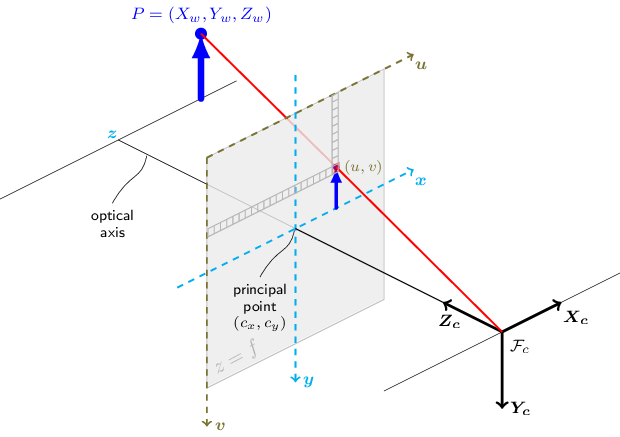
\includegraphics[width=0.7\textwidth]{figures/pinhole_camera_model.png}
    \caption{Camera model and various coordinate systems~\cite{opencv_calib3d}}
\end{figure}

The objective of solving the PnP problem can be described as finding a rigid body transform $\mathbf{T}_{wc}$ from the world reference frame $\mathcal{F}_w$ to the camera reference frame $\mathcal{F}_c$. A pinhole camera model is assumed, and 3D points $\mathbf{P}_w$ are mapped to the image plane in two steps. First, a point $\mathbf{P}_w$ is mapped to a point in the camera reference frame $\mathbf{P}_c$ via the camera to world transform $\mathbf{T}_{cw}$. Second, $\mathbf{P}_c$ is mapped to a pixel $\mathbf{p}$ through a projective transform and the camera intrinsic matrix $\mathbf{K}$. The full transformation from $\mathbf{P}_w$ to $\mathbf{p}$ can be described by the mapping below.
\begin{gather*}
    s\mathbf{p}=\mathbf{K} \onebytwo{\mathbf{R}_{cw}}{\mathbf{t}_{cw}}\mathbf{P}_w \\
    s \begin{bmatrix}x \\ y \\ 1\end{bmatrix} = \begin{bmatrix}f_x & 0 & c_x \\ 0 & f_y & c_y \\ 0 & 0 & 1\end{bmatrix} \begin{bmatrix} r_{11} & r_{12} &  r_{13} & t_{1} \\ r_{21} & r_{22} &  r_{23} & t_{2} \\ r_{31} & r_{32} &  r_{33} & t_{3} \end{bmatrix} \begin{bmatrix} X_w \\ Y_w \\ Z_w \\ 1 \end{bmatrix}
\end{gather*}

All 2D and 3D points are represented in homogenous coordinates. $\mathbf{K}$ is the camera intrinsic matrix where $f_x$, $f_y$ are focal lengths and $c_x$, $c_y$ represents the translation to camera center (since image coordinates are generally defined from the top left). $\onebytwo{\mathbf{\mathbf{R}}_{cw}}{\mathbf{\mathbf{t}}_{cw}}$ represents the composition of the camera to world transform $\mathbf{\mathbf{T}}_{cw}$ followed by a projective transform $\onebytwo{\mathbf{\mathbf{I}}_{3 \times 3}}{\mathbf{\mathbf{0}}}$ mapping from 3D space to the 2D image plane.
\begin{align*}
    \onebytwo{\mathbf{R}_{cw}}{\mathbf{t}_{cw}} = \onebytwo{\mathbf{I}_{3 \times 3}}{\mathbf{0}} \twobytwo{\mathbf{R}_{cw}}{\mathbf{t}_{cw}}{\mathbf{0}}{1}
\end{align*}

Lastly, $s$ is an arbitrary scale parameter representing the scale ambiguity introduced by the projective transform. In other words, all 3D points on a given ray from the camera center will map to a single 2D point on the image plane. $s$ also covers the scale ambiguity from using homogenous representations.

In the PnP problem the camera is calibrated, therefore $\mathbf{K}$ is known. The camera pose $\mathbf{T}_{wc}$ has 6 DoF (3 translational + 3 rotational), so at least 3 point correspondences (2 DoF per point) are required for a solution. However, there can be up to four solutions for the P3P problem, so a 4th point is needed in practice to disambiguate. 

\subsection{2D robot pose}
\label{section:robot_pose}

\begin{figure}
    \centering
    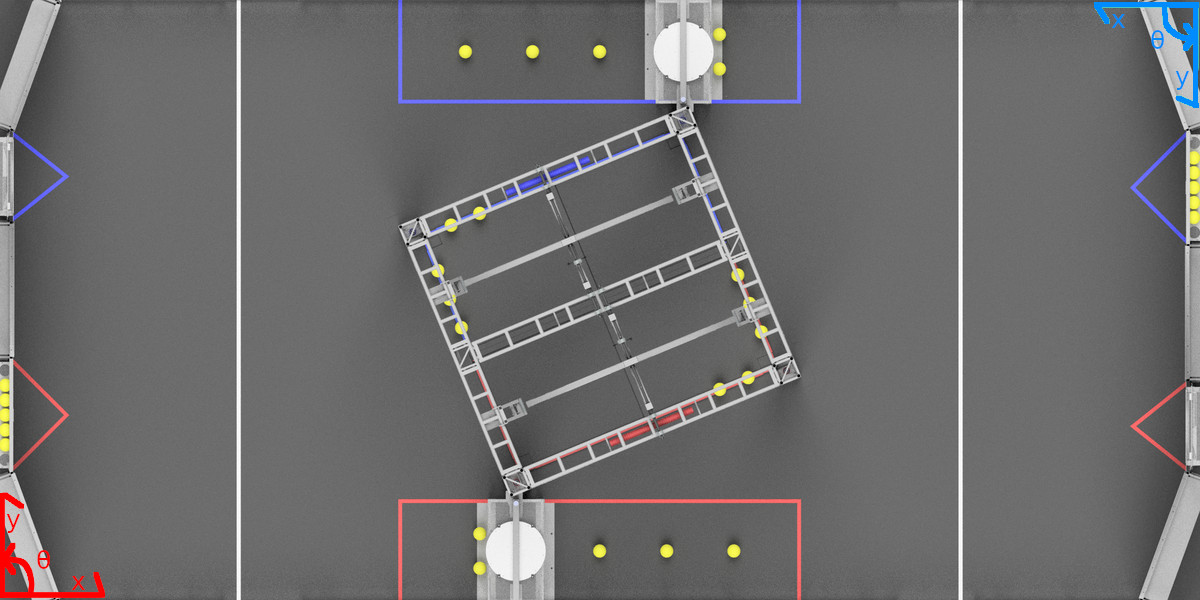
\includegraphics[width=0.5\textwidth]{figures/infinite-recharge.jpeg}
    \caption{Typical field coordinate system (origin is at bottom-left corner for red alliance)~\cite{wpilib_geom}}
\end{figure}

While the camera pose $\mathbf{T}_{wc}$ is a 3D transformation, the field-relative robot pose is typically represented as a 2D field to robot transformation $\mathbf{X}_{fr}$. To determine the robot pose, the 2D world to camera transformation $\mathbf{X}_{wc}$ must first be calculated from the camera pose:
\begin{gather*}
    x_{wc}=Z_{wc} \qquad y_{wc}=-X_{wc} \qquad \theta_{wc}=-\alpha_{wc} \\
    \mathbf{X}_{wc} = \begin{bmatrix} \cos\theta_{wc} & -\sin\theta_{wc} & x_{wc} \\ \sin\theta_{wc} & \cos\theta_{wc} & y_{wc} \\ 0 & 0 & 1\end{bmatrix}
\end{gather*}

Then $\mathbf{X}_{fr}$ can be calculated using the 2D field to world transformation $ \mathbf{X}_{fw}$ and 2D camera to robot transformation $\mathbf{X}_{cr}$:
\begin{equation*}
    \mathbf{X}_{fr} = \mathbf{X}_{fw}\mathbf{X}_{wc}\mathbf{X}_{cr}
\end{equation*}

\subsection{Direct Linear Transformation (DLT)}
The DLT is used to solve a set of $n$ similarity relations $s_k \mathbf{x}_k = \mathbf{A} \mathbf{y}_k$. $\mathbf{x}_k$ and $\mathbf{y}_k$ are known vectors, $\mathbf{A}$ is an $m \times n$ matrix of unknowns and $s_k$ is an arbitrary non-zero scalar. The minimum number of equations required to solve for $\mathbf{A}$ is $m \times n - 1$.

\section{OpenCV solvePnP}
By default OpenCV's \verb|cv.solvePnP()| method uses the \verb|cv.SOLVEPNP_ITERATIVE| algorithm~\cite{opencv_calib3d}. First, the camera to world translation $\mathbf{t}_{cw}$ (\verb|tvec|) and axis-angle rotation $\mathbf{r}_{cw}$ (\verb|rvec|) are approximated using the point correspondences and the DLT. Second, nonlinear optimization of these parameters is used to minimize the reprojection error of the world points onto the image.

\subsection{Camera to world transform via the DLT}
\label{section:dlt}

Since $\mathbf{K}$ is known, the camera model equation can be rewritten in terms of 2D normalized image points $\mathbf{p}_c$ and $3 \times 4$ transformation matrix $\mathbf{Q}$~\cite{dlt}.
\begin{gather*}
    \mathbf{p}_c=\mathbf{K}^{-1}\mathbf{p} \\
    \mathbf{Q}=\onebytwo{\mathbf{R}_{cw}}{\mathbf{t}_{cw}} \\
    s\mathbf{p}_c=\mathbf{Q}\mathbf{P}_w
\end{gather*}

In the general case with a non-planar target, solving for $\mathbf{Q}$ using the DLT requires at least 11 equations to determine all the matrix entries. This requires 6 point correspondences even though there are only 6 DoF in the unknown camera pose.\footnotemark{} Once $\mathbf{Q}$ has been obtained, it can be partitioned into $\mathbf{R}_{cw}$ and $\mathbf{t}_{cw}$.

\footnotetext{Sometimes in practice, only 4 or 5 non-planar points are available. In this case, alternative algorithms such as ePnP are commonly employed to approximate $\mathbf{T}_{cw}$. Such algorithms solve for the 6 camera pose DoF directly rather than the unknown parameters in $\mathbf{Q}$.}

In the case of a planar target, the world points all have the same $Z_w$ coordinate. Because of this, the DLT can no longer be used to determine the entries of $\mathbf{Q}$ directly.\footnote{The resulting coefficient matrix $\mathbf{M}$ constructed in DLT has $\dim (\mathcal{N} ( \mathbf{M} ) ) > 1$ so a unique solution cannot be determined for $\mathbf{Q}$.} A workaround is to ignore $Z_w$ and the 3rd column in $\mathbf{Q}$. The problem can then be reformulated using 2D world points $\mathbf{p}_w$ and $3 \times 3$ homography matrix $\mathbf{H}$.
\begin{gather*}
    \mathbf{p}_w=\begin{bmatrix}X_w & Y_w & 1\end{bmatrix}^T \\
    \mathbf{H} = \begin{bmatrix} r_{11} & r_{12} & t_{1} \\ r_{21} & r_{22} & t_{2} \\ r_{31} & r_{32} & t_{3} \end{bmatrix} \\
    s\mathbf{p}_c=\mathbf{H}\mathbf{p}_w
\end{gather*}

Solving for $\mathbf{H}$ using the DLT requires at least 8 equations to determine all the matrix entries, so 4 point correspondences are needed. Once $\mathbf{H}$ has been found, it can be decomposed into $\mathbf{R}_{cw}$ and $\mathbf{t}_{cw}$ using Zhang's SVD-based method~\cite{zhang}. Alternatively, OpenCV offers \verb|cv.decomposeHomographyMat()| which implements an analytical decomposition algorithm~\cite{malis2007deeper}. Lastly, $\mathbf{R}_{cw}$ is converted to an axis-angle rotation $\mathbf{r}_{cw}$ using Rodrigues' formula.

\subsection{Nonlinear optimization of camera to world transform}
\label{section:nonlinear_optimization}

Solving for $\mathbf{T}_{cw}$ using the DLT minimizes a linear cost function. However, this cost function does not have a physical interpretation. In addition, the decomposition of $\mathbf{H}$ into $\mathbf{R}_{cw}$ and $\mathbf{t}_{cw}$ is only approximate. Thus, it is important to refine the DLT solution for an accurate camera pose.

Reprojection error is used to optimize $\mathbf{r}_{cw}$ and $\mathbf{t}_{cw}$. First, $\mathbf{r}_{cw}$ is converted back to $\mathbf{R}_{cw}$ using Rodrigues' formula. Next, world points $\mathbf{P}_w$ are reprojected onto the image frame as $\mathbf{\hat{p}}$. Finally, the distance between these reprojected points and the original image points $\mathbf{p}$ is minimized using Levenberg–Marquardt and the least squares cost function below.
\begin{gather*}
    \hat{\mathbf{p}}=\mathbf{K}\onebytwo{\mathbf{R}_{cw}}{\mathbf{t}_{cw}}\mathbf{P}_w \\
    \min_{\mathbf{r}_{cw},\mathbf{t}_{cw}} \quad \sum_{k=1}^{n}{||\mathbf{p}^{(k)}-\mathbf{\hat{p}}^{(k)}(\mathbf{r}_{cw},\mathbf{t}_{cw})||^2}
\end{gather*}

After a local minimum is reached, a refined $\mathbf{r}_{cw}$ and $\mathbf{t}_{cw}$ are returned. These can be used to compute camera pose and robot pose using the formulas in \ref{section:pnp} and \ref{section:robot_pose}. OpenCV also provides \verb|cv.solvePnPRefineLM()| to perform the refinement step independently.

\section{Mobile robot pose estimation using vision target}
The PnP formulation covers the general case of camera pose estimation for $n \geq 3$ point correspondences. However, when estimating mobile robot pose using a vision target, additional assumptions can often be made to improve pose accuracy.

\subsection{Infinitesimal plane-based pose estimation (IPPE)}
PnP makes no assumptions about the planarity of the world points. However, vision targets  are often on flat surfaces such as walls or signs. In this case, \verb|cv.SOLVEPNP_IPPE| can be used to approximate $\mathbf{r}_{cw}$ and $\mathbf{t}_{cw}$ instead of the method described in \ref{section:dlt}. IPPE improves on the DLT approach by considering where the homography transform is most accurate and solving for the camera pose around this point~\cite{ippe}. Like the DLT method, the result from IPPE can be used to initialize the nonlinear optimization detailed in \ref{section:nonlinear_optimization}. However, since IPPE provides a more accurate estimate, the optimization can generally be solved in fewer iterations. In particular, this combination is often used with AR targets such as ArUco markers.

\subsection{Modified nonlinear optimization of camera pose}
PnP also assumes that the camera can be located anywhere in 3D space. However, in the scenario of interest, the camera is rigidly attached to a mobile robot. The task space of this robot is a horizontal plane, and the vision target is at a fixed height relative to the plane. This means that the height $Y_{wc}$, pitch $\beta_{wc}$ and roll $\gamma_{wc}$ of the camera are fixed. The nonlinear optimization described in \ref{section:nonlinear_optimization} can be modified as follows to keep these parameters constant.

First, the transformation matrix can be rewritten in terms of the camera yaw, pitch, roll and XYZ translation:
\begin{align*}
    \onebytwo{\mathbf{R}_{cw}}{\mathbf{t}_{cw}} = \mathbf{R}_{wc} \onebytwo{\mathbf{I}_{3 \times 3}}{-\mathbf{t}_{wc}} = \mathbf{R}_y(\alpha_{wc}) \mathbf{R}_x(\beta_{wc}) \mathbf{R}_z(\gamma_{wc}) \onebytwo{\mathbf{I}_{3 \times 3}}{\begin{matrix}-X_{wc} \\ -Y_{wc} \\ -Z_{wc}\end{matrix}} 
\end{align*}

Then a new minimization problem can be constructed in terms of the camera pose rather than $\mathbf{r}_{cw}$ and $\mathbf{t}_{cw}$. This can also be solved using Levenberg–Marquardt, holding $Y_{wc}$, $\beta_{wc}$ and $\gamma_{wc}$ constant.
\begin{gather*}
    \hat{\mathbf{p}}=\mathbf{K} \mathbf{R}_y(\alpha_{wc}) \mathbf{R}_x(\beta_{wc}) \mathbf{R}_z(\gamma_{wc}) \onebytwo{\mathbf{I}_{3 \times 3}}{\begin{matrix}-X_{wc} \\ -Y_{wc} \\ -Z_{wc}\end{matrix}}  \mathbf{P}_w \\
    \min_{\alpha_{wc}, X_{wc}, Z_{wc}} \quad \sum_{k=1}^{n}{||\mathbf{p}^{(k)}-\mathbf{\hat{p}}^{(k)}(\alpha_{wc}, X_{wc}, Z_{wc})||^2}
\end{gather*}

Even if $Y_{wc}$, $\beta_{wc}$ and $\gamma_{wc}$ cannot be determined reliably from physical measurements or CAD models, they can be calibrated ahead of time by averaging several measurements from a standard PnP algorithm. These values can then be treated as constants and re-calibrated as necessary.

\bibliographystyle{unsrt}
\bibliography{refs}

\end{document}